\documentclass[draftclsnofoot,onecolumn,letterpaper,10pt]{IEEEtran}

\usepackage{geometry}
\geometry{textheight=9.5in, textwidth=7in}

\usepackage{float}
\usepackage{graphicx}
\usepackage{algorithm2e}
\usepackage{pgfgantt}
\usepackage{booktabs}
\graphicspath{ {images/} }

\newcommand{\subparagraph}{}
\usepackage{titlesec}

\begin{document}
\begin{center}
	{\huge\textbf{Senior Software Engineering Design Group 7}}
	\vspace{1cm}

	{\Huge\textbf{brew.ai Progress Report -- Winter Term}}

	\vspace{2cm}
	\textbf{Connor Yates}\\yatesco@oregonstate.edu

	\textbf{Aravind Parasurama}\\parasura@oregonstate.edu

	\textbf{Cody Holliday}\\hollidac@oregonstate.edu

	\vspace{2cm}
	{\Large CS 462, Winter 2017}
	\vspace{1cm}
\end{center}

\begin{abstract}

\end{abstract}

\newpage
\tableofcontents
\newpage

\section{Purposes and Goals}
\subsection{Project Purpose}
Brew.ai is a hardware and software solution for automated brewing of mead or beer.
Currently, home brewing requires a lot of time, knowledge, and patience.
As such, it is not accessible to amateurs, and brew.ai seeks to solve this problem.
From amateurs to professional brewers, we want brew.ai to be useful by automating the brewing process and helping brewers make better tasting products.

\subsection{Project Goals}
At the end of the project, we look to produce a physical device that contains the necessary electronics and software to control the brewing process.
The brew.ai device itself is a bucket lid that will fit over a brewing device and have various modules incorporated in it.
The lid device will monitor and control temperature, send and receive commands/data to and from the Android application, and monitor fermentation status.
From the perspective of a user, setup will be essentially plug-and-play.
No technical knowledge is needed beyond knowing how to pair a Bluetooth device an Android device, open an app, and put ingredients into a bucket.
brew.ai also will improve on its recipe over time by leveraging the power of reinforcement learning and the users own feedback on the product it creates.
A main goal of this project is creating a product with the ability to learn from each batch, and improve its performance.

\section{Current Project Status}
In general, brew.ai is slightly behind schedule. Recently, we have procured all the hardware necessary to create our brewing device, and coding has been started on the AI and UI sections. Even with this progress, there are still many things to be done, and the separate components still need to be completed and integrated.
We will need to concentrate effort on this project in the coming weeks to bring it back up to schedule so it may be seen to a successful conclusion.

\subsection{Hardware\\{\em\textbf{Aravind Parasurama}}}
\subsubsection{Overview}
brew.ai hardware is modular, flexible, and scalable.
The current testing hardware is a generic large mason jar with a tight-sealing
electronic lid, however the brew.ai platform can easily work with setups ranging
from what is used for testing to a professional brewing operation with multiple
brews being automated.
The hardware components can be categorized as the microcontroller element, and
everything else.
For this demo, the microcontroller of choice is the AVR ATmega32u4, which provides
us with a nice range of GPIO, PWM and ADC pins to work with when broken out.
The completed AVR routine will execute commands received from the AI, and send
sensor data to the AI.
Sensors are plug-and-play as per the user's discretion, however the crucial elements
for operation are the heating and cooling element, the water table sensor, and
the thermometer.
As the heating element requires a lot of power for continous operation, the brew.ai
hardware will require a consistent power source.

\subsubsection{Current Status}
The hardware is shaping up to be a safely housed microcontroller unit with support
for plug-and-play functionality with a variety of sensors relevant to brewing. \\
At this time, the microcontroller supports operating a heating element, the water
table sensor, and a stirring element.
The microcontroller routine receieves key-value packets over USART, with the keys
indicating which operation needs to be executed.
The microcontroller will also periodically read and send data from a temperature
module, a pH sensor, and a digital hydrometer of some sort.
Microcontroller code is entirely written in C, with the platform of choice being
AVR.
For easy plug-and-play functionality, a number of AVR libraries for interfacing
with i2c and SPI. \\
The current testing hardware is a large glass mason jar, with electronic components
like the microcontroller, thermometer and ultrasonic sensor fashioned into the lid.
The heating element protrudes from the lid, and the magnetic stirring element
is attached to the bottom.

\subsubsection{Tasks Left}
The hardware portion of the project has some work to go.
A reliable and easily reproducible method of measuring fermentation needs to be made.
A 3D printed enclosure needs to be designed for the testing hardware to be usable.
More testing hardware also needs to be created, so that there can be a nice demo in May.
As the current protoype cycle is ending, professional feedback on current brewing progress
needs to be sought.

\subsubsection{Roadblocks}
Implementing hardware from design resulted in a lot of roadblocks.
Finding a reliable, food safe heating element has been difficult.
The current solution to that is to repurpose water heater elements, however those
are not reputed for their food safety.
Measuring fermentation has also been problematic.
Traditionally, in home brewing, a brewer would measure fermentation by measuring
the change in specific gravity of the solution over time.
Unfortunately, the process of measuring specific gravity is analog, and there does
not exist a low-cost, simple way of digitally measuring specific gravity with a
sensor.
The current proposed solution for this is to incorporate an ultrasonic sensor to
detect the waterlevel over set intervals.
The change in the water table should indicate progress in fermentation.
To more accurately measure the fermentation process, the hardware will also need
to incorporate pH sensing, carbon sensing, and ethanol sensing.

\subsection{Android Interface\\{\em\textbf{Cody Holliday}}}
Currently there has been little progress on the development of the interface, however since the device can be controlled through a command ilne interface, this does not impede us from testing the AI or the hardware.


\subsubsection{Work Done and Roadblocks}
Since the User Interface has fallen on me to complete, there has been little done in the way of creating a testing skeleton.
All of the roadblocks have been due to lack of time on my part. Especially week 6 which started off with my birthday
and Valentines day and ended with two midterms.
My current solution to my lack of time is to take an incomplete in one of my heavier courses so that I can focus on the development of the User Interface.
Currently I have one way communication from the Android to my laptop. I can connect my phone to my
computer, then input text into a text field and send it to the computer where a python script captures and prints the string.
Here are the screenshots of my current progress.

\newpage
\vfill

\begin{figure}
\label{fig:layout}
\caption{Here is the layout of the app currently.}
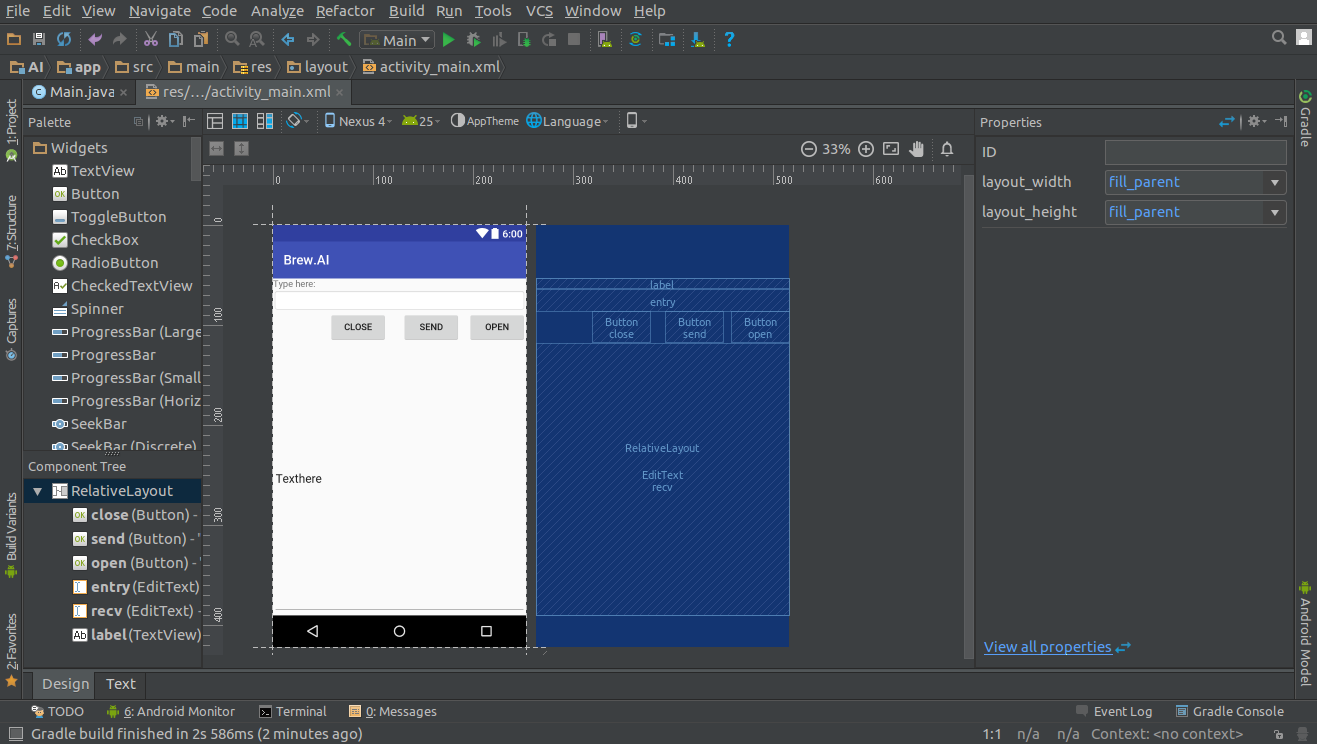
\includegraphics[scale=0.4]{android-layout.eps}
\end{figure}


\begin{figure}
\label{fig:code}
\caption{This is some of the code for button functionality.}
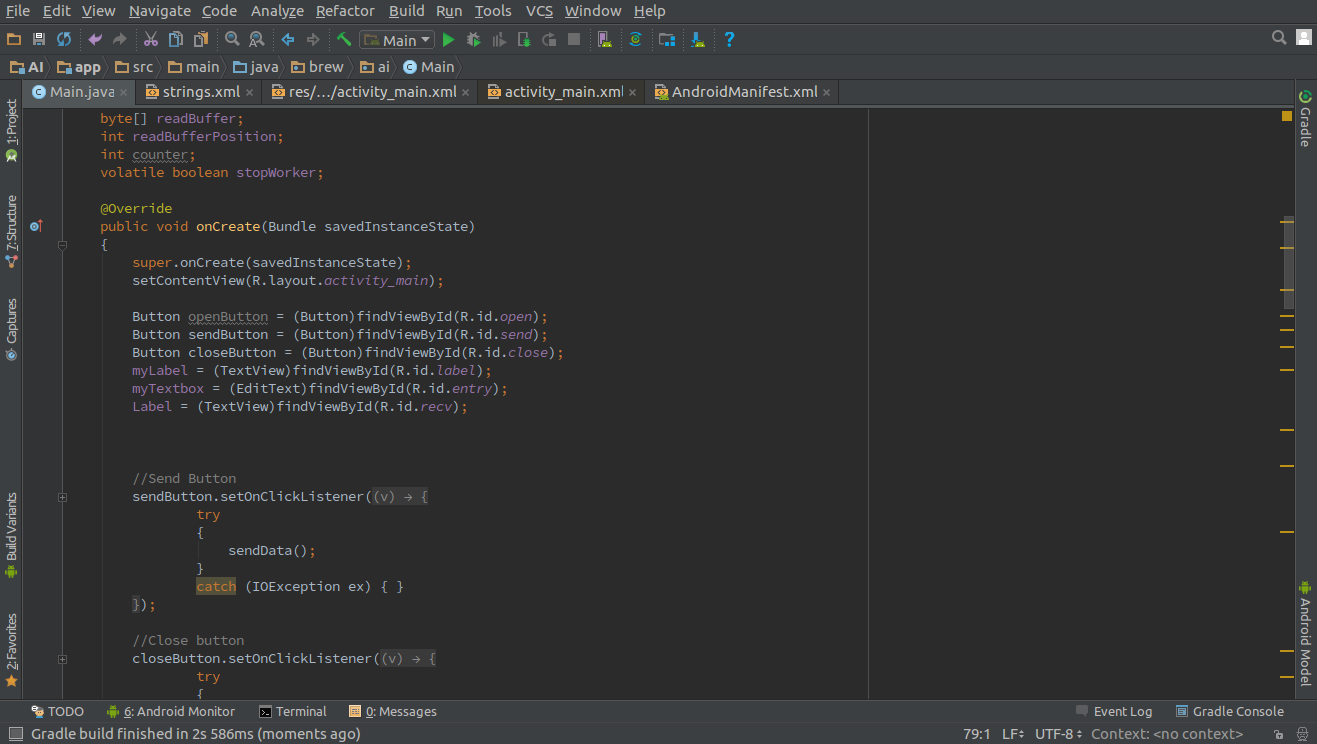
\includegraphics[scale=0.4]{android-code.eps}
\end{figure}


\begin{figure}
\label{fig:python}
\caption{This is the python script written to transmit and receive information.}
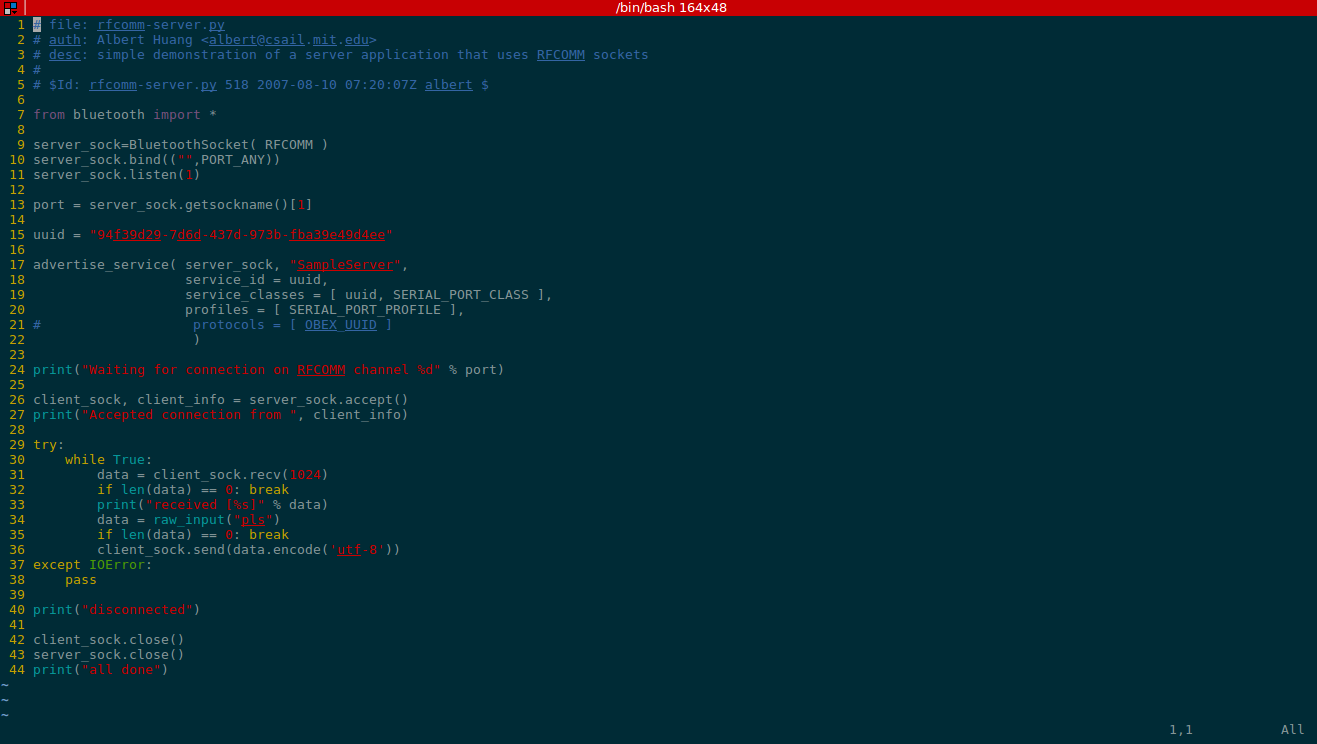
\includegraphics[scale=0.4]{python-server.eps}
\end{figure}

\vfill
\clearpage
\subsubsection{Work Left Undone}
My first goal is to create two way Bluetooth communication between the controller and the Android device.
To implement two way communication I need to write a message handler that can listen and receive messages on a Bluetooth socket.
Once this is finished I need to test it on the Raspberry Pi and make sure it interfaces with Bluetooth correctly.
There may be differences between how Raspian Linux and Ubuntu Linux handle Bluetooth sockets, but this should be
a minor change if needed.


After the Bluetooth communication is fully implemented, then we can begin on developing the control protocol.
The Raspberry Pi and the Android device will exchange messages in a simple text format separated by non-letter characters.
Data from the brewing process will be formatted in a JSON object as part of this string.
The Android device will put this data into an object, then use the Graphview Android library to plot the data on the Android Device.
I will also need to develop the interface between the Bluetooth listener on the controller and the AI itself.
This should be as simple as using control structures in the main program and an asynchronous listener to handle messages from the Bluetooth connection.
The final part of the app development will be making this as an app that a user can download on their phone.
This will allow us to offer a less expensive version of the product without the Android device interface.
Currently the Python side looks specifically for my phone, but it can be generalized to support other devices.
This app would be free on the Google Play store as a companion product to the Brew.AI device.

\subsubsection{App Design}
The app design will be simple with as little steps between starting and brewing as possible.
Four options are available on the home screen: Brew For Me, Let Me Brew, Data, and Settings.
The Brew For Me button will take the user to a screen that contains a list of ingredients as well as amounts.
Once the user has checked off each of those ingredients, the start button becomes available to the user to press to start brewing.
The Let Me Brew button is similar to the Brew For Me button, but gives the user control of the amounts of each of the ingredients.
After the ingredients screen a process screen comes up listing all the different variables in the brewing process.
The screen will have default or suggested numbers for these variables, but the user can alter these as they wish.


At this point for both buttons the user is prompted to add flavorings to the batch and log what they put in.
Once the user is done with ingredients and process settings, brewing begins.
The last two buttons are data, and settings. The data button takes the user to another screen where they can see data from all the batches they have ever brewed.
The data will be presented in two forms: a graph of all the data from each batch combined, and each batch separately.
This will include graphs over time of how each batch changed, much like how it is shown during the brewing process.
The settings button will give the user control over the visual aspect of the app and allow them to enable usability options.
Other features would include clearing the brewing data off the Android to prevent it from becoming full, but the data sets will probably be small and take up kilobytes of space on the phone.


\subsection{Artificial Intelligence\\{\em\textbf{Connor Yates}}}
\subsubsection{AI Review and Purpose}
The artificial intelligence aspect of this project is to create an autonomous agent which watches over the brewing process.
The agent will have the ability to read data from sensors immersed in the brew, and act upon its decisions.
Available actions are a stirring element, a heating element, and a trigger to stop the brewing process.

Instead of hand-coding a specific policy based on historical data, we elected to use reinforcement learning.
Specifically, we will use Q-learning with experience replay to train a neural network to gauge what actions should be taken when presented with a representation of the world.
Q-learning traditionally uses a table to store Q-values for a finite set of state-actions pairs.
We will represent our brewing process as a 4-dimensional state storing the current temperature, specific gravity, $CO_2$ level, and time.
These variables are continuous, and have a potentially infinite range.
Instead of attempting to manually bin their continuous domain into a discreet one, we will use a neural network to stand in place of the Q-table.
Neural networks are general function approximators, and have been shown to be able to approximate the function encoded by the Q-table.
This method will provide the structure for an intelligent, autonomous agent which learns from its environment.

In order to test the performance and robustness of the AI, we are considering creating a simple simulator of a brewing system, based on simple physics principles.
This system will allow us to create basic, but meaningful test data with which to train the AI on.
The need for this secondary system is not yet cemented, but I will be proceeding as if it is needed.
T


\subsubsection{AI Progress}
The artificial intelligence agent is moving along well, but could be more finished.
The neural network is implemented, and its input/output interfaces have been tested.
However, work is needed to complete the reinforcement learning algorithms which will give the AI the power to learn.

The code base is still small, under 100 lines.
This is attributed mostly to the use of the Keras library, which allows me to create the neural network in a handful of lines.
From there, I have been working on implementing the Q-value update function, which allows the agent to learn.
Simultaneously, I am working on implementing the experience replay algorithm, which influences the way ``experiences'' are pulled for the Q-value update function.
Experience replay works by storing recent experiences (state-reward pairs) and selecting from that memory during training.
This way, a single experience can be used during learning more than once, and can help encode time dependent structures in the neural net.

Once this code is completed, it will be very short, around 250 lines at the most. The use of Python and robust neural network libraries helps keep the codebase small. Additionally, the algorithms themselves are not long; just complicated.
To finish writing the AI, I will need to complete the Q-update function (which updates the neural network) and implement the experience replay algorithm.

After this functionality is completed, the next step will be to write an execution loop using the interface provided by the Teensy microcontroller.
This execution loop will read data from the microcontroller to create a state for the neural network to process.
The neural network will generate an action to take, which is sent back to the microcontroller to be executed in the brewing system.

\subsubsection{Simple Simulator}
In order to test the learning parameters and ability of the neural network to learn a Q-value function, I will consider writing a small simulator for brewing process.
This will be a simple model of the system, as writing code to actually model chemical interactions would be prohibitively difficult.
Instead, the simulator will provide update the state of the system using a combination of simple functions.
For example, temperature changes can be simply modeled as increasing when the heating element is on, and cooling when it is not.
The rate of the change is given by the simple temperature differential equations.
The specific gravity will simply modeled as a linear function of time, since sugars are converted to alcohol in a one-way fashion.
By creating a simple simulator of the system and training to hit a specific curve through the state space, we can see how effectively and quickly the agent is able to learn a brewing process.

If there are any errors or inconsistencies in this basic learning phase, this can be used to refine the agent design into a better working agent for the task of brewing.

\subsubsection{Roadblocks and Solutions}
As it stands, there are no major technical or intellectual blocks to completing this section of the project.
I understand the math behind Q-Learning and experience replay (which are the two main aspects of the AI).
I also have designed and begun implementation on a Python class structure which would allow me to train an agent, once we have data.
However, even with an understanding of the theoretical aspects of the reinforcement learning techniques, this is my first time writing code to implement Q-learning.
This new-to-me implementation of the algorithm is contributing to the slowdown I see on my section of the project.
While there is not much code to write, it is very precise and careful code which I am writing.

The main delay in completing the AI has been time.
Between research duties, grad school applications, and homework loads, free time this term has been few and far between.
However, the second half of the term will be better in this regard. This week our research team finished a project for a journal, which was ongoing for the last few months.
Additionally, I will be demoting my grading status for one of my classes this term, as it is just for fun.
This will allow me to reallocate time from that class to this project.

I believe the AI section has, at most, 20 hours of coding work before it is completed.
Subsequently, finishing this section of the project should happen soon
This will allow me to help my teammates with their sections, as well as keep on top of the planning needed to create a successful expo presentation.


\section{Summary}
The brew.ai project, while currently behind schedule, is succeeding where technical aspects of the project are involved.
The weakness currently delaying the project is not technical in nature, but rather is an issue of time management and balancing the work of this project with other commitments.
This is heartening, as it presents a very clear solution to our current problem: sit down and schedule priorities, and see where time can be shifted toward this project.
Even with this issue of time management, we are confident the project will continue to move forward and be completed on time.
With no major technical aspects blocking our progress, the way forward is relatively well defined. All that remains is to walk that path.

\end{document}
